\subsection{Robustness to Non-Uniform Within-Bin Subgroup
  Distributions}
\label{sec:app_within}

Our bounds on the full sample CEF $E(y|x)$ (See Section~\ref{ssec:math} and Appendix \ref{app:robust}) rely on the uniformity of the rank distribution, which is given when working with a national sample. However, when working with population subsamples (e.g. Muslims), uniformity is not guaranteed. Take the example of the 1960s, where 57\% of fathers are in the lowest education bin. Conditional on being in the bottom bin, the distribution of latent ranks of Muslim fathers is \textit{not} necessarily uniform.

This lack of uniformity creates a potential bias. For example, approximately 10\% of the fathers in the bottom education bin are Muslims. If the latent ranks of these fathers were all concentrated at the bottom of the bin, and the latent ranks of Hindus were concentrated at the top of the bin, then the mobility gap between Hindus and Muslims would be biased upward. In other words, the gap in son outcomes between Hindus and Muslims could be driven not only by a difference in outcomes conditional on father education rank, but also by unobserved differences in the latent father ranks.

The extent of bias is determined by the extent to which the within-bin latent education rank distribution for each subgroup differs from the uniform distribution and how that difference changes over time. In this section, we present three pieces of evidence that these departures do not substantially bias our primary results.

First, we examine whether there is substantial socioeconomic divergence between SCs and Muslims in the parent generation, using additional data. The evidence rejects a large enough change to explain the SC/Muslim mobility divergence. Second, we show that the divergence of upward mobility between Scheduled Castes and Muslims is found even when we rank parents according to their position in the education distribution of their own subgroup---given this ranking, the latent rank distribution within each bin is guaranteed to be uniform, eliminating the bias threat (at the cost of calculating a slightly less useful mobility statistic). Third, we use parametric assumptions to estimate the latent rank distribution suggested by the distribution of education completion across bins. We show that the maximal bias under a range of parametric assumptions is very small and unlikely to affect our conclusions.

The issues addressed in this appendix are not unique to our analysis, but are implicit in any comparison of groups that conditions on education levels. However, our discussion of latent education ranks makes this concern particularly visible.

\subsubsection{Socioeconomic Changes for Muslims and SCs in Parent Generations}
\label{sec:muslim_sc_other_diffs}

Figure~\ref{fig:sc_muslim_ses_trends} shows time series plots with various socioeconomic indicators representing the parent generation of our sample. We focus on SC and Muslim outcomes, as we aim to test the hypothesis that changes in relative positions at the bottom of the socioeconomic distribution drive the relative mobility changes documented for these groups in the paper. Panel A and B show education levels and ranks of the \textit{parents} of the 1950--89 birth cohorts. Muslim parents have higher education in all years; there is a partial convergence of about one rank point --- equivalent to less than half a year of education --- between the two groups. A convergence of this size is far too small to explain the 7 rank point (or $\sim$1.5 years of education) that has opened between bottom-half children in these groups.

However, these estimates are from the full distribution of parents; perhaps Muslims at the bottom of the distribution have done relatively worse than those at the top. We cannot, of course, compare education changes in the bottom half of the distribution, since they are entirely bottom-coded. We therefore turn to household consumption, looking at individuals aged 40--60 in NSS samples from 1983--2012.\footnote{To our knowledge, the 1983 NSS is the earliest electronically available NSS with per capita consumption recorded. 2012 is the last NSS survey year available. If fathers are 20--30 when their children is born, this set of surveys covers the parents of birth cohorts ranging from 1943--1992, thus approximately covers the parents of children in our main sample.} We limit the sample to individuals in the bottom half of the education distribution in their cohort/year. Panel C shows the log consumption gap between Muslims and Forwards/Others, and the same gap between SCs and Forwards/Others, from 1983--2012. Panel D shows the same result in terms of consumption ranks. The gaps are largely stable over the sample period; there is no evidence that bottom-half Muslims have lost ground to members of Scheduled Castes over the sample period.

In short, there is little evidence to suggest that Muslim bottom-half parents of the 1980s were particularly negatively selected as compared to Muslim bottom-half parents of the 1950s or 1960s cohorts.

\begin{figure}[H]
  \caption{Trends in Socioeconomic Status for Muslims and SCs in Parent Generations}
  \label{fig:sc_muslim_ses_trends}

  \begin{center}
    \begin{tabular}{cc}
      
      \panel{A. Years of Education (IHDS parents)} &
      \panel{B. Education Rank (IHDS parents)}    \\ 
      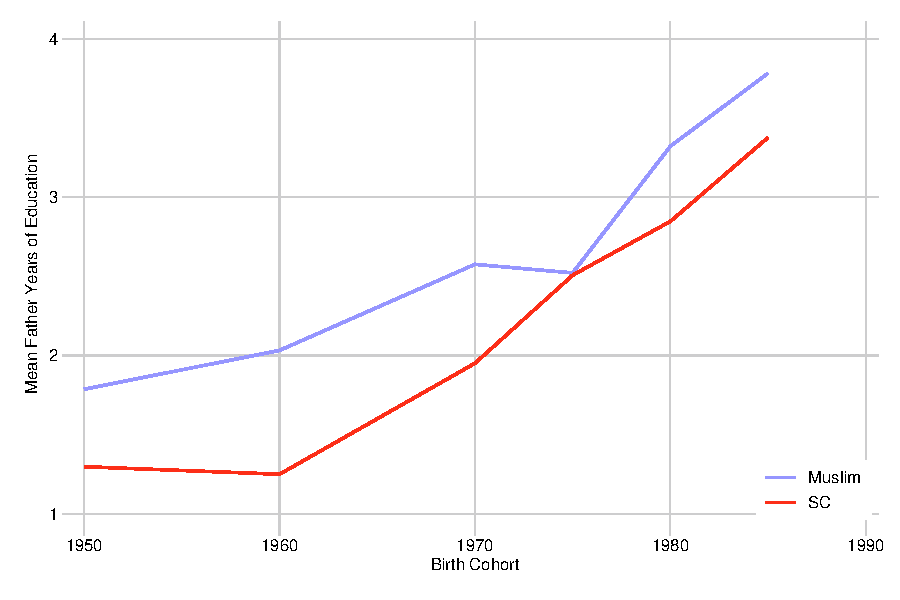
\includegraphics[scale=0.55]{\mobilitypath/sc_mus_father_years} &
      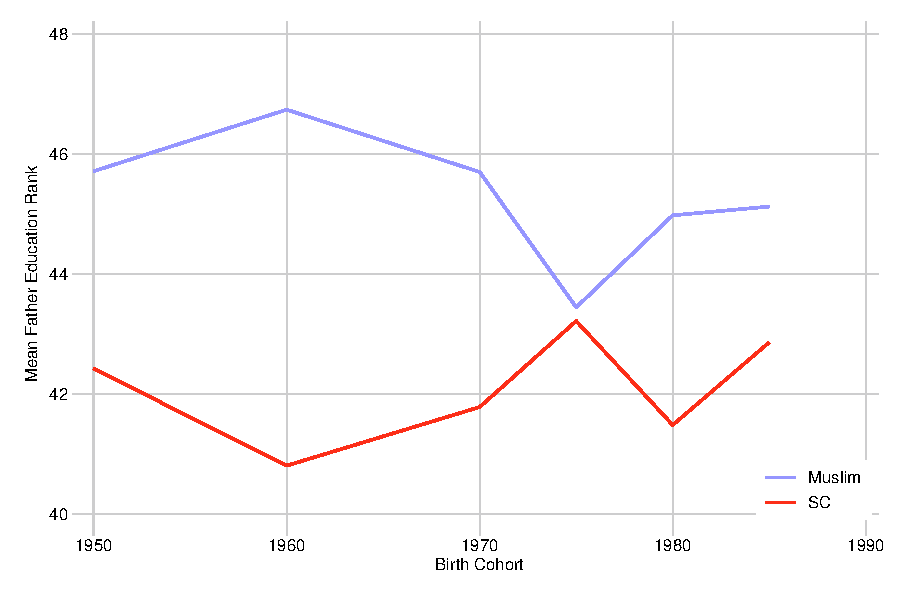
\includegraphics[scale=0.55]{\mobilitypath/sc_mus_father_ranks}
      \\
      
      \panel{C. Log Consumption Gap      vs. Forwards/Others (NSS Households)} &
      \panel{D. Log Consumption Rank Gap vs. Forwards/Others (NSS Households)}    \\ 
      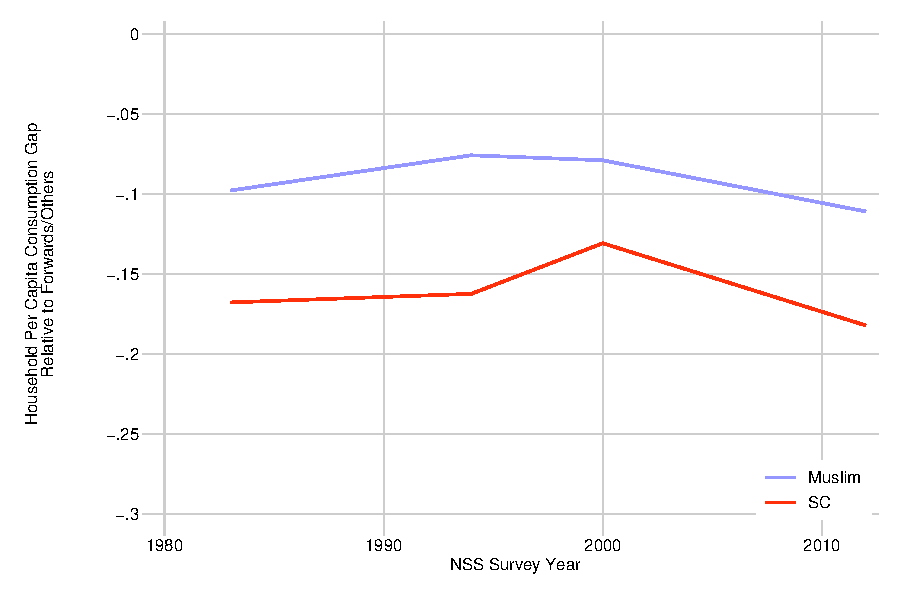
\includegraphics[scale=0.55]{\mobilitypath/mpce_low_line} &
      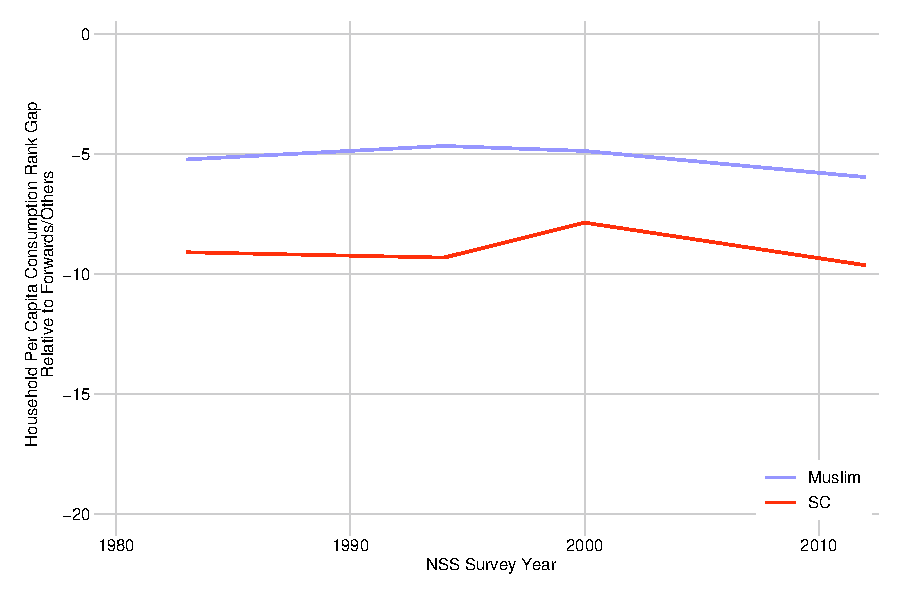
\includegraphics[scale=0.55]{\mobilitypath/mpce_rank_low_line}
      \end{tabular}          
  \end{center}
  \newline
  \footnotesize{\singlespace Figure \ref{fig:sc_muslim_ses_trends} shows trends in socioeconomic status of SCs and Muslims. Panels A and B present education levels (years) and within-cohort education ranks for the \textit{parents} of male respondents in the birth cohorts on the X axis. Ranks are calculated using the midpoint rank of education bins. Panel C uses household-level NSS data to show the log consumption gap between Muslims and Forwards/Others (blue) and SCs and Forwards/Others (red), for households where the head is aged 30--50 and \textit{is in the bottom half of the education distribution.} The X axis shows the NSS survey year. Panel D shows the consumption rank gaps for the same surveys/groups. Source: IHDS (2012), NSS (1983--2012).}
\end{figure}

\clearpage

\subsubsection{Using Within-Subgroup Rank Distributions which are Uniform by Construction}
\label{sec:app_rank_within}

We show here that the Muslim-SC mobility divergence is robust to calculating parent ranks \textit{within} subgroups. Under this rank definition, latent parent ranks within each subgroup are uniform by construction---the latent ranks of SCs in the bottom 50\% of SCs must be uniformly distributed. This fully resolves the non-uniform bias problem, but the cost of making this assumption is that we are no longer comparing groups with similar levels of education---the least educated 50\% of SCs have a lower level of education than the least educated 50\% of Forwards and thus cannot be expected to attain the same outcomes even if there are no cross-group outcome differences after controlling for parent education. For this reason, we use national ranks in the body of the paper. Note that SC and Muslim parents have similar levels of education (much more similar than their children, see Figure~\ref{fig:sc_muslim_ses_trends}), making the latter concern less important here as well.

Figure \ref{fig:subgroup_within_ranks} shows the result. Panel A repeats the result of Figure~\ref{fig:group_mob} for Forwards/Others, Muslims, and SCs, using national ranks, showing changes in upward mobility ($\mu_0^{50}$) over time for each group. Panel B shows the same result, with parent ranks calculated within their own subgroups. The bounds in Panel B are too wide to distinguish mobility changes between SCs and Muslims, because the within-rank bottom-coding problem is more severe among the marginalized groups, where the parent generation is less educated. More than 70\% of SC parents in the 1960s report a bottom-coded education level, resulting in wide bounds on $\mu_0^{50}$ for this rank definition. 

To tighten the bounds, we instead estimate $\mu_0^{70}$: the expected child outcome given a parent in the bottom 70\% of the parent education distribution. Panel C shows $\mu_0^{70}$ calculated using national ranks, as in the body of the paper. Panel D shows $\mu_0^{70}$ calculated using own-subgroup ranks, as in Panel B. The divergence of SCs and Muslims, and the convergence of SCs and Forwards/Others is sustained in both of these panels. The level gap between SCs/Muslims and Forwards/Others is higher in Panels B and D because the bottom X\% of SCs/Muslims represent lower levels of education than the bottom X\% of Forwards/Others, whereas Panels A and C hold parent education constant.

The consistency of these results with parent ranks calculated within subgroups (which are uniform by construction) strongly suggests that our primary results are not driven by differential unobserved changes in the latent parent rank distributions of the individual subgroups.

%%%%%%%%%%%%%%%%%%%%%%%%%%%%%%%%%%%%%%%%%%%%%%%%%%%%%%%
%% ROBUSTNESS TO ALTERNATE SUBGROUP RANK DEFINITIONS %%
%%%%%%%%%%%%%%%%%%%%%%%%%%%%%%%%%%%%%%%%%%%%%%%%%%%%%%%
\begin{figure}[H]
  \caption{Subgroup Upward Mobility (Fathers/Sons):
    \cnewline National Ranks vs. Within-Subgroup Ranks} 
  \label{fig:subgroup_within_ranks}

  \begin{center}
    \begin{tabular}{cc}
      
      \panel{A. Fathers ranked in national distribution $\mu_0^{50}$} &
      \panel{B. Fathers ranked in subgroup distribution $\mu_0^{50}$}    \\ 
      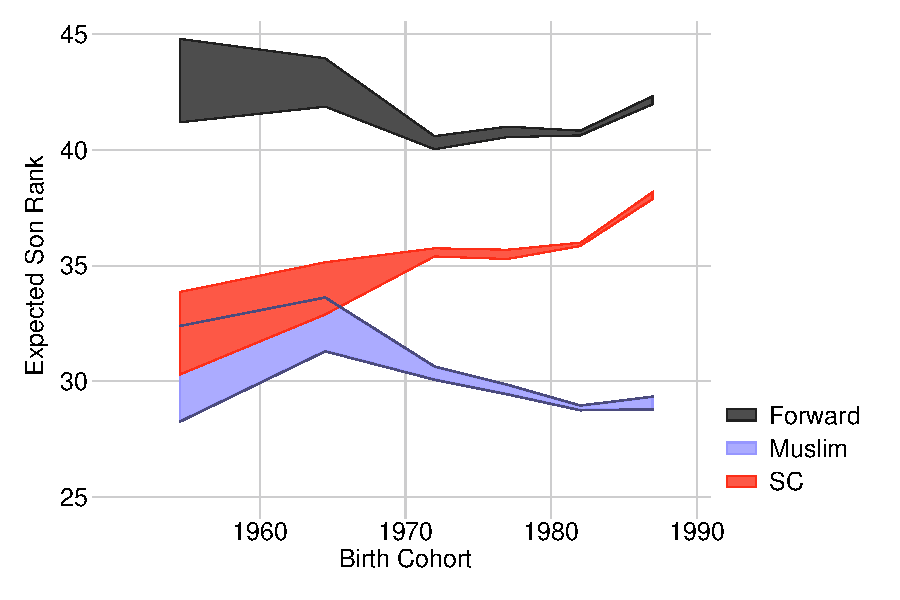
\includegraphics[scale=0.55]{\mobilitypath/ihds_mob_group_across_mu50} &
      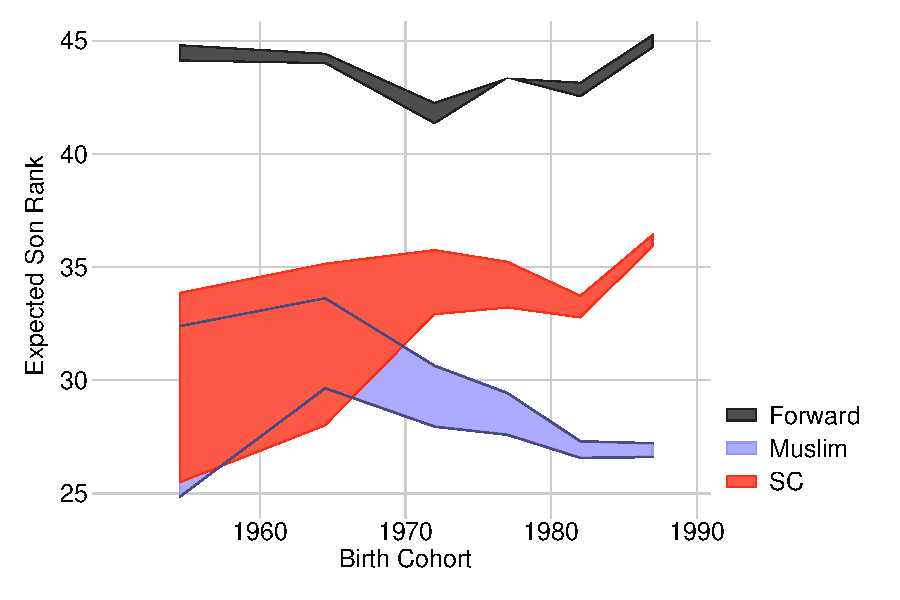
\includegraphics[scale=0.55]{\mobilitypath/ihds_mob_group_within_mu50}
      \\
      
      \panel{C. Fathers ranked in national distribution $\mu_0^{70}$} &
      \panel{D. Fathers ranked in subgroup distribution $\mu_0^{70}$}    \\ 
      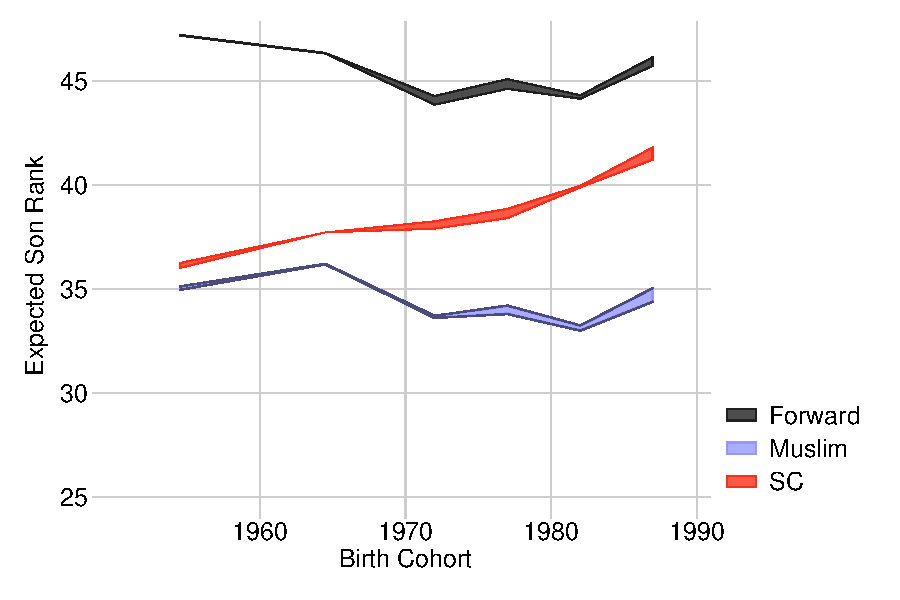
\includegraphics[scale=0.55]{\mobilitypath/ihds_mob_group_across_mu70} &
      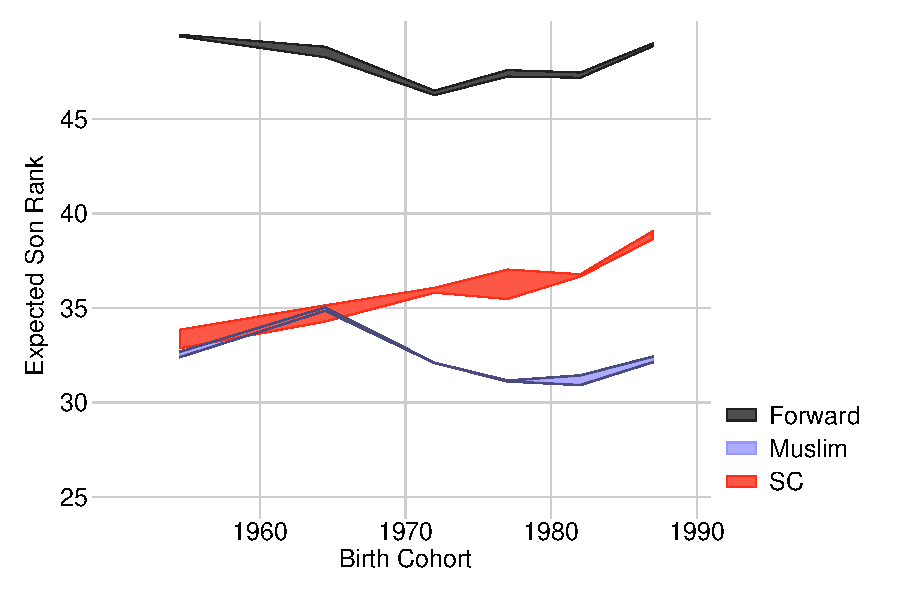
\includegraphics[scale=0.55]{\mobilitypath/ihds_mob_group_within_mu70}
      \end{tabular}          
  \end{center}
  \newline
\footnotesize{\singlespace Figure \ref{fig:subgroup_within_ranks} shows trends in upward mobility for Forward/Others, Muslims, and SCs. Panel A presents bottom-half mobility by ranking fathers in the national distribution, as in the body of the paper. Panel B ranks fathers within each subgroup, recovering uniformity by construction. Panels C and D are similar to A and B, except they present bounds on $\mu_0^{70}$ (i.e., average son rank, conditional on being born to a father in the bottom 70\%) rather than $\mu_0^{50}$. } 
\end{figure}


\subsubsection{Inferring Latent Education Ranks Using Parametric Assumptions}
\label{sec:app_parametric}

This section takes an alternate route to modeling the unobserved variation at the bottom of the education distribution. We assume that the latent rank distribution takes a parametric form (normal or lognormal); we then estimate the full distribution using the cross-bin education distribution for every group.

These parameterized distributions let us produce a continuous latent rank distribution for each subgroup. In the body of the paper, we assumed this distribution was uniform for each group within each bin. The parameterizations let us predict separate within-bin latent rank distributions for each group, based on each group's full distribution of education. We can compare these predicted latent distributions to the uniform distribution used in the paper to gauge the extent of bias that could arise from the uniformity assumption.

For each population subgroup, we fit a normal and a lognormal distribution to the sample distribution of years of education. We then create a simulated population that has the same proportion of each subgroup as the true population, and for each individual, we draw their years of education from the fitted parametric distribution. This gives us a continuous education distribution that matches the moments from the discrete sample distribution.  Finally, we transform the years of education variable into ranks with respect to the entire population. This gives us a simulated population with continuous ranks.

We focus on the 1960--69 and 1985--89 cohorts, as we aim to check the validity of our conclusion that Muslim and SC mobility have diverged over this period.

Table~\ref{tab:sim_moments} compares the moments from the IHDS sample with the moments from the simulated distributions. Here, we are ignoring children and only examining how far the parent latent rank distribution \textit{across groups} differs from what we would get from the uniformity assumption.

For both the 1960--69 and the 1985--89 birth cohorts, the simulated moments are close matches to the raw data. The group ordering and approximate gaps between groups is preserved; the standard deviation of the simulated data is slightly higher than that of the true binned data, which is to be expected, given the truncation of the binned data.

\begin{table}
    \begin{center}
      \caption{Actual and Simulated Moments from the Education Rank Distribution}
      \label{tab:sim_moments}
      \small{
      
\begin{tabular}{rcc|cccc}
\multicolumn{7}{c}{A. 1960-1969 Birth Cohort} \\[0.25ex]
\hline
\hline
& \multicolumn{2}{c|}{\textul{Binned Data}} &  \multicolumn{4}{c}{\textul{Simulated
  Distributions}} \\[0.25ex]
& \multicolumn{2}{c|}{ } &  \multicolumn{2}{c}{Normal} &  \multicolumn{2}{c}{Lognormal} \\[0.25ex]
\hline
& Mean & SD & Mean & SD & Mean & SD \\[0.25ex]
Forward / Other &
55.2 & 26.8 &
55.8 & 30.1 &
55.9 & 29.4 \\[0.25ex]
Muslim &
46.7 & 24.5 &
46.6 & 27.4 &
46.2 & 28.1 \\[0.25ex]
Scheduled Castes &
40.8 & 21.0 &
39.6 & 23.0 &
39.7 & 24.6\\[0.25ex]
Scheduled Tribes &
39.1 & 20.2 &
38.5 & 23.3 &
37.7 & 23.9\\[0.25ex]
\hline
\hline
\\
\\
\multicolumn{7}{c}{B. 1985-1989 Birth Cohort} \\[0.25ex]
\hline
\hline
& \multicolumn{2}{c|}{\textul{Binned Data}} &  \multicolumn{4}{c}{\textul{Simulated
  Distributions}} \\[0.25ex]
& \multicolumn{2}{c|}{ } &  \multicolumn{2}{c}{Normal} &  \multicolumn{2}{c}{Lognormal} \\[0.25ex]
\hline
& Mean & SD & Mean & SD & Mean & SD \\[0.25ex]
Forward / Other &
56.5 & 27.6 &
56.5 & 28.6 &
56.6 & 27.9 \\[0.25ex]
Muslim &
45.1 & 26.7 &
44.8 & 27.5 &
45.4 & 28.2 \\[0.25ex]
Scheduled Castes &
42.9 & 26.7 &
42.8 & 27.5 &
42.6 & 28.1\\[0.25ex]
Scheduled Tribes &
35.6 & 25.0 &
36.1 & 24.9 &
34.9 & 26.1\\[0.25ex]
\hline
\hline
\end{tabular}
}
    \end{center}
Table \ref{tab:sim_moments} shows the mean and standard deviation of the true data (IHDS), compared with the mean and standard deviation of simulated distributions, split by demographic subgroup.
  \end{table}  

In Table~\ref{tab:sim_param_ranks}, we use the simulated data to examine the
distribution of the latent variable \textit{within} the bins where our
method assumed uniformity in the main analysis. Specifically, we examine the mean parent
education rank conditional on being in the bottom 50\%. As expected,
parents from less educated social groups have lower latent ranks even
after conditioning on being in the bottom 50\%.\footnote{If the
  subgroup distributions were all uniform within this bin, then all
  groups would have a mean rank of 25.} However, the
differences are very small, and they do not change much from the
1960--69 to the 1985--89 birth cohorts, under any of the
distributional assumptions. Even in the worst case scenario (the
lognormal distribution with constant variance), the gap between Muslim
and SC parents in the bottom 50\% shrinks from 2.5 to 1, a 1.5
percentage point change.

\begin{table}
  \begin{center}
  \caption{Simulated Average Parent Rank Conditional on Rank $\leq$ 50}
  \label{tab:sim_param_ranks} 
  \small{\begin{tabular}{rcc|cc}
\multicolumn{5}{c}{A. 1960-1969 Birth Cohort} \\[0.25ex]
\hline
\hline
& \multicolumn{2}{c|}{\textul{Group-level Variance}} &  \multicolumn{2}{c}{\textul{Constant Variance}}\\[0.25ex]
& \multicolumn{1}{c}{Normal} & \multicolumn{1}{c|}{Lognormal}  & \multicolumn{1}{c}{Normal}  & \multicolumn{1}{c}{Lognormal}  \\[0.25ex]
\hline
Forward / Other & 24.4 & 25.4 & 27.0 & 27.2 \\[0.25ex]
Muslim & 24.9 & 24.1 & 24.3 & 24.5 \\[0.25ex]
Scheduled Castes & 26.0 & 24.9 & 22.6 & 22.2 \\[0.25ex]
Scheduled Tribes & 25.2 & 24.3 & 21.8 & 21.9 \\[0.25ex]
\hline
\hline
\\
\\
\multicolumn{5}{c}{B. 1985-1989 Birth Cohort} \\[0.25ex]
\hline
\hline
& \multicolumn{2}{c|}{\textul{Group-level Variance}} &  \multicolumn{2}{c}{\textul{Constant Variance}}\\[0.25ex]
& \multicolumn{1}{c}{Normal} & \multicolumn{1}{c|}{Lognormal}  & \multicolumn{1}{c}{Normal}  & \multicolumn{1}{c}{Lognormal}  \\[0.25ex]
\hline
Forward / Other & 26.6 & 27.6 & 27.5 & 27.2 \\[0.25ex]
Muslim & 24.4 & 24.0 & 24.1 & 24.4 \\[0.25ex]
Scheduled Castes & 23.7 & 23.2 & 23.2 & 23.3 \\[0.25ex]
Scheduled Tribes & 22.8 & 21.1 & 21.0 & 21.1 \\[0.25ex]
\hline
\hline
\end{tabular}
}
  \end{center}
Table \ref{tab:sim_param_ranks} presents the simulated average parent rank conditional on being in the bottom half of the distribution under two parametric distributions (normal and lognormal). The left panel estimates distribution mean and variance separately for each demographic subgroup; the right panel uses the same variance for each distribution, estimated from all the data.
\end{table}  

Given the average CEF slope of 0.5, this suggests that changing latent
parental status within the coarse education bins can explain at most
0.75 rank points of the growing difference between Muslims and
SC/STs. Under other distributional assumptions the potential bias is
even smaller. In comparison, our midpoint estimate of this change from
1960--69 to 1985--89 in the body of the paper is 7.4 rank points. This is not a strict upper bound, because child outcomes could be correlated with latent ranks, something we do not address here. But the scale of the effect on the average rank difference conditional on being in the bottom half strongly suggests that non-uniformity within bins is not a major factor explaining our results.

In short, we consider it unlikely that changing parental position
within observed rank bins can explain the growing mobility gap between
SCs and Muslims. All the evidence brought to bear suggests that the relative positions of these groups within the bottom education
bins has not changed enough to substantially bias our
group-level estimates.

% \subsection{Robustness to Adjusting for Censored Child Ranks}
% \label{sec:app_child_censoring}
% 
% In the main part of the paper, we focus on bounding a function $Y(x) =
% E(y|x)$ when $y$ is observed without error, but $x$ is observed with
% interval censoring. In this section, we modify the setup to consider
% simultaneous interval censoring in the conditioning variable $x$ and
% in observed outcomes $y$. In the mobility context, this
% double-censoring setup arises when the $y$ variable is a child rank
% (as in Figure~\ref{fig:mu_gender}A and \ref{fig:mu_gender}B), but not
% when the $y$ variable is a child level of education (as in
% Figure~\ref{fig:mu_gender}C and \ref{fig:mu_gender}D). As noted in the
% paper, all of our results are consistent whether we use levels or
% ranks as outcomes. We nevertheless proceed here to examine the
% potential bias from ignoring the censoring of child ranks.
% 
% One approach to this problem would be to use a problem setup similar
% to that presented in Section~\ref{sec:method}, that takes into account
% the information on child ranks that is lost by binning. We developed a
% numerical optimization that could bound the CEF by searching over all
% possible joint distributions of latent $x$ and $y$ variables, but with
% $n^2$ the number of parameters compared with the single-censoring
% model, it proved computationally infeasible.
% 
% We therefore present two alternate approaches to the problem here.
% First, we define the latent distributions of $y$ variables that would
% generate the maximal and minimal mobility statistic in theory. We can
% then bound the mobility statistic following our standard method under
% these best- and worst-case assumptions. This union of these bounds is
% a very conservative bound on the mobility statistic given censoring in
% both the $y$ and $x$ variables.
% 
% Second, we can shed light on the distribution of the true average
% value of $y$ in each $x$ bin if other data is available. This approach
% is feasible whenever more information is available about children than
% about their parents, as is the case in our context (and in many
% others).  Specifically, we use data on child wages to predict whether
% the true latent child rank distribution ($y$) is better represented by
% the best- or worst-case mobility scenario. The joint wage distribution
% suggests that the true latent distribution of $y$ in each bin is very
% close to the best case distribution, which we used in
% Section~\ref{sec:results}.
% 
% % , because there is little effect of parent
% % education on child wages after conditioning on child education.
% 
% \subsubsection{Best and Worst Case Mobility Distributions}
% \label{sec:best_worst}
% 
% In this section, we take a sequential approach to the double-censoring
% problem. We first calculate the set of child CDFs for each level of
% parent education that would correspond to the highest and lowest
% possible intergenerational mobility. From these CDFs, we can calculate
% the average latent rank of children in each parent bin. These may be
% different from the latent rank implied by assigning each child the
% midpoint of their bin. With these latent ranks, we can then follow the
% estimation procedure outlined in Section~\ref{sec:method}. This gets
% us a wider set of bounds that takes the censoring of child ranks into
% account.
% 
% To make the example concrete, consider two children who have less than
% 2 years of education; one is from a rich family and one is from a poor
% family. Assume that 20\% of children in the population have less than
% 2 years of education. In the body of the paper, we would assume that
% each of these children has a rank of 10 (i.e. the midpoint of the
% bottom bin). But it is possible that the child from a poor family has
% a latent rank of 7 and the child from a rich family has a latent rank
% of 13. In this case, mobility would be lower than what we have
% measured in the paper.
% 
% Given that child rank is known only to lie in one of $h$ bins,
% there are two hypothetical scenarios that describe the best and worst
% cases of intergenerational mobility. Mobility will be lowest if child
% outcomes are sorted perfectly according to parent outcomes
% \textit{within} each child bin, and highest if there is no additional
% sorting within bins.\footnote{Specifically, these scenarios
%   respectively minimize and maximize both the rank-rank gradient and
%   $\mu_0^{x}$ for any value of $x$. To minimize and maximize $p_x$, a different
%   within-bin arrangement is required for every $x$. We leave this out
%   for the sake of brevity, and because bounds on $p_x$ are minimally
%   informative even with uncensored $y$.}
% 
% Note that the case of perfect sorting within bins fits very poorly
% with the standard human capital model. In this model, the binned
% education data reflects a continuous demand for education with a lumpy
% number of years available for purchase. It is difficult to theorize a
% distribution where there is a large mass of rich children bunched just
% below a bin boundary, and no rich children just above that boundary.
% Given that children of rich and poor parents appear in every bin in
% the child distribution, the true distribution is likely to be closer
% to the uniform case than the perfectly ordered case.  Note also that
% we do not consider the case of perfectly reversed sorting, where the
% children of the least educated parents occupy the highest ranks within
% each child rank bin, as it would violate the stochastic dominance
% condition (and is implausible).
% 
% Appendix Figure~\ref{fig:son_solution} shows two set of CDFs that
% correspond to these two scenarios for the 1960--69 birth cohort.  In
% Panel A, children's ranks are perfectly sorted according to parent
% education within bins. Each line shows the CDF of child rank, given
% some father education. The points on the graph correspond to the
% observations in the data---the value of each CDF is known at each of
% these points and thus the CDFs must pass through them.  Children below
% the 27th percentile are in the lowest observed education bin. Within
% this bin, the CDF for children with the least educated parents is
% concave, and the CDF for children with the most educated parents is
% convex---indicating that children from the best off families have the
% highest ranks within this bin. This pattern is repeated within each
% child bin.  The implausibility of this scenario is reflected by the
% kinked nature of these CDFs, which are unlikely to appear in the real
% world. Panel B presents the high mobility scenario, where children's
% outcomes are uniformly distributed within child education bins, and
% are independent of parent education within child bin.
% 
% Each of these CDFs can be collapsed to a single mean child rank for
% each parent bin. From these expected child ranks, we can then use the
% method from Section~\ref{sec:method} to calculate bounds on any
% mobility statistic. The top two rows of Table~\ref{tab:double_censor}
% shows bounds on $\mu_0^{50}$ and on the rank-rank gradient for the
% high and low mobility scenarios.  Taking censoring in the child
% distribution into account widens the bounds on all parameters. The
% effect is proportionally larger for bottom half mobility, because it
% was so precisely estimated before---the bounds on $\mu_0^{50}$
% approximately double in width when censoring of son data is taken into
% account.
% 
% These bounds are very conservative, as the worst case scenario is
% implausible, as noted above. In the next subsection, we draw on
% additional data on children, which suggests that the best case
% mobility scenario is close to the true joint latent distribution.
% 
% \subsubsection{Estimating the Child Distribution Within Censored Bins}
% 
% Because we have additional data on children, we can estimate the shape
% of the child CDF within parent-child education bins using rank data
% from other outcome variables that are not censored. Under the
% assumption that latent education rank is correlated with other
% measures of socioeconomic rank, this exercise sheds light on whether
% Panel A or Panel B in Figure~\ref{fig:son_solution} better describes
% the true latent distribution.
% 
% Figure~\ref{fig:son_wage_cdf} shows the result of this exercise using wage data
% from men in the 1960s birth cohort. To generate this figure, we
% calculate children's ranks first according to education, and then
% according to wage ranks within each education bin.\footnote{We limit
%   the sample to the ~50\% of men who report wages. Results are similar
%   if we use household income, which is available for all
%   men. Household income has few missing observations, but in the many
%   households where fathers are coresident with their sons, it is
%   impossible to isolate the son's contribution to household income
%   from the father's, which biases mobility estimates downward.} The
% solid lines depict this uncensored rank distribution for each father
% education; the dashed gray lines overlay the estimates from the high
% mobility scenario in Panel B of Figure~\ref{fig:son_solution}.
% 
% If parent education strongly predicted child wages \textit{within}
% each child education bin, we would see a graph like Panel A of
% Figure~\ref{fig:son_solution}. The data clearly reject this
% hypothesis. There is some additional curvature in the expected
% direction in some bins, particularly among the small set of
% college-educated children, but the distribution of child cumulative
% distribution functions is strikingly close to the high mobility
% scenario, where father education has only a small effect on
% child wage ranks after child education is taken into account. The last
% row of Table~\ref{tab:double_censor} shows mobility estimates using
% the within-bin parent-child distributions that are predicted by child
% wages; the mobility estimates are nearly identical to the high
% mobility scenario. This result suggests that our assumption in
% Section~\ref{sec:results} that the latent child rank is the midpoint of
% the rank bin for all parent groups is not affecting our estimates very
% much.
% 
% Note that there is no comparable exercise that we can conduct to
% improve upon the situation when parent ranks are interval censored,
% because we have no information on parents other than their education,
% as is common in mobility studies. 
% 
% Note finally that the potential bias from assuming uniformity within
% child rank bins is increasing in the size of the rank bins. Because
% children are more educated than parents in every cohort, this bias is
% smaller for children than it would be for parents. It is also smaller
% for the younger cohorts of children born in the 1980s than it is for
% the example we used here.
% 
% %%%%%%%%%%%%%%%%%%%%%%%%%%%%%%
% %% BEGIN APPENDIX C FIGURES %%
% %%%%%%%%%%%%%%%%%%%%%%%%%%%%%%
% {\singlespacing
% \begin{figure}[H]
% 
%   \caption{Best- and Worst-Case Son CDFs \cnewline by Father Education (1960-69
%     Birth Cohort)}
%   \label{fig:son_solution}
% 
%   \begin{center}
%     \begin{tabular}{c}
% 
%       Panel A: Lowest Feasible Mobility
%       \\
%       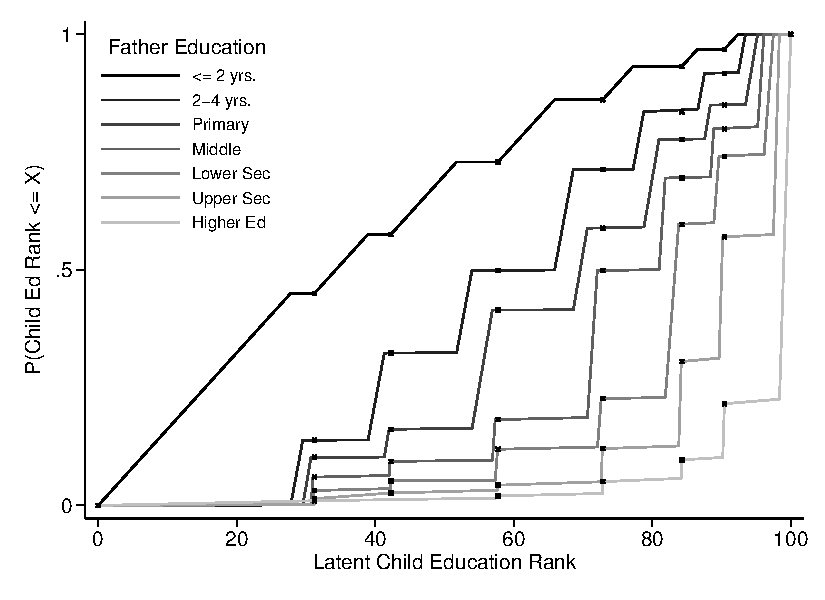
\includegraphics[scale=0.80]{\mobilitypath/cdf_low_mob} \\
%       \\
%       \\
%       Panel B: Highest Feasible Mobility
%       \\
%       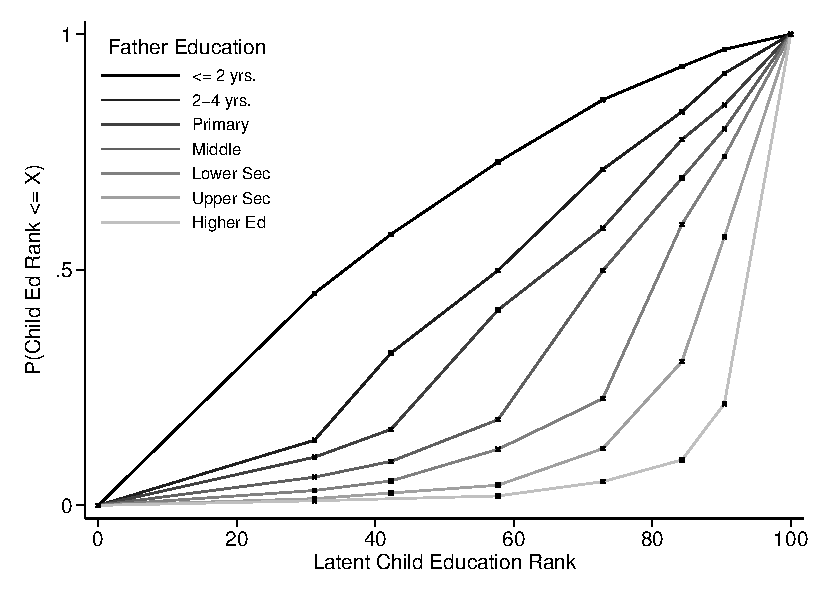
\includegraphics[scale=0.80]{\mobilitypath/cdf_high_mob} \\
% 
%     \end{tabular}
%     \hline
%   \end{center}
% 
%   { \footnotesize Figure~\ref{fig:son_solution} shows a set child CDFs
%     conditional on each level of father education that correspond to
%     the best and worst case scenarios for intergenerational
%     mobility. The lines index father types. Each point on a line shows
%     the probability that a child of a given father type obtains an
%     education rank less than or equal to the value on the X axis in
%     the national education distribution. The large markers show the
%     points observed in the data.}
% 
% \end{figure}
% 
% \begin{figure}[H]
%   \caption{Son Outcome Rank CDF \cnewline
%     by Father Education (1960-69 Birth
%     Cohort) \cnewline {\small Joint Education/Wage Estimates}} 
%   \label{fig:son_wage_cdf}
%   \begin{center}
%     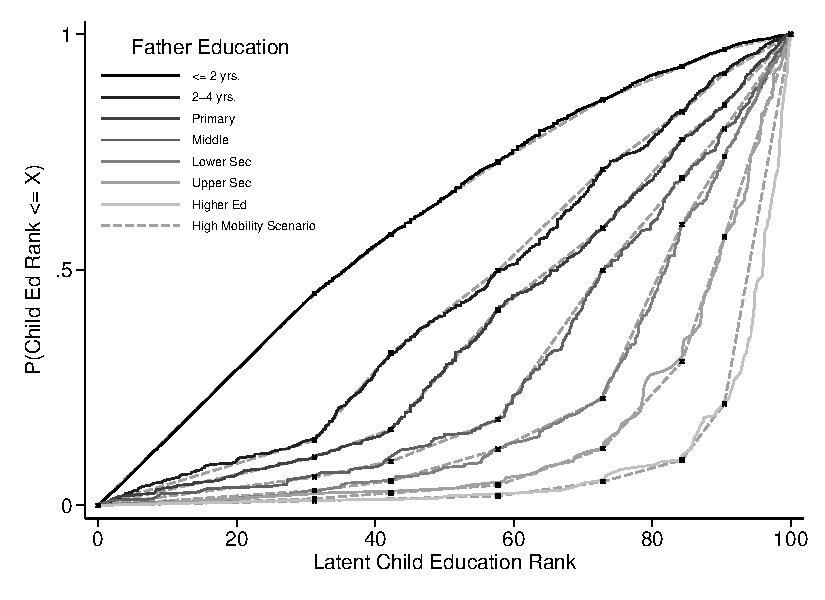
\includegraphics[scale=0.80]{\mobilitypath/cdf_combined}
%     \hline
%   \end{center}
%       {\small Figure~\ref{fig:son_wage_cdf} plots a son rank
%         CDF separately for each father
%         education level, for sons born in the 1960s in India. Sons
%         are ranked first in terms of education, and then in terms of
%         wages. Sons not reporting
%         wages are dropped. For each father type, the graph shows a
%         child's probability of attaining less than or equal to the
%         rank given on the X axis.}
% \end{figure}
% 
% \floatbarrier
% 
% \begin{table}[H]
%   \caption{Mobility Estimates under Double-Censored CEF }
%   \label{tab:double_censor} 
%   \begin{tabular}{lcc}
\hline\hline
  &  Upward Interval          &  Rank-Rank \\
  & Mobility ($\mu_0^{50}$)  &  Gradient ($\beta$)        \\
Low mobility scenario &   [32.33, 35.90]          &  [0.55, 0.80]  \\
High mobility scenario &  [35.86, 38.80]      &  [0.45, 0.67]  \\
Wage imputation scenario &  [35.79, 38.70]     &  [0.46, 0.67]  \\

\hline
\end{tabular}


% \end{table}  
% \footnotesize{Table \ref{tab:double_censor} presents bounds on
%   $\mu_0^{50}$ and the rank-rank gradient $\beta$ under
%   three different sets of assumptions about child rank distribution
%   within child rank bins. The low mobility scenario assumes children
%   are ranked by parent education within child bins. The high mobility
%   scenario assumes parent rank does not affect child rank after
%   conditioning on child education bin. The wage imputation predicts the
%   within-bin child rank distribution using child wage ranks and parent
%   education.}
% 
% }
